\documentclass[twoside]{book}

% Packages required by doxygen
\usepackage{fixltx2e}
\usepackage{calc}
\usepackage{doxygen}
\usepackage[export]{adjustbox} % also loads graphicx
\usepackage{graphicx}
\usepackage[utf8]{inputenc}
\usepackage{makeidx}
\usepackage{multicol}
\usepackage{multirow}
\PassOptionsToPackage{warn}{textcomp}
\usepackage{textcomp}
\usepackage[nointegrals]{wasysym}
\usepackage[table]{xcolor}

% NLS support packages
\usepackage{polski}
\usepackage[T1]{fontenc}

% Font selection
\usepackage[T1]{fontenc}
\usepackage[scaled=.90]{helvet}
\usepackage{courier}
\usepackage{amssymb}
\usepackage{sectsty}
\renewcommand{\familydefault}{\sfdefault}
\allsectionsfont{%
  \fontseries{bc}\selectfont%
  \color{darkgray}%
}
\renewcommand{\DoxyLabelFont}{%
  \fontseries{bc}\selectfont%
  \color{darkgray}%
}
\newcommand{\+}{\discretionary{\mbox{\scriptsize$\hookleftarrow$}}{}{}}

% Page & text layout
\usepackage{geometry}
\geometry{%
  a4paper,%
  top=2.5cm,%
  bottom=2.5cm,%
  left=2.5cm,%
  right=2.5cm%
}
\tolerance=750
\hfuzz=15pt
\hbadness=750
\setlength{\emergencystretch}{15pt}
\setlength{\parindent}{0cm}
\setlength{\parskip}{3ex plus 2ex minus 2ex}
\makeatletter
\renewcommand{\paragraph}{%
  \@startsection{paragraph}{4}{0ex}{-1.0ex}{1.0ex}{%
    \normalfont\normalsize\bfseries\SS@parafont%
  }%
}
\renewcommand{\subparagraph}{%
  \@startsection{subparagraph}{5}{0ex}{-1.0ex}{1.0ex}{%
    \normalfont\normalsize\bfseries\SS@subparafont%
  }%
}
\makeatother

% Headers & footers
\usepackage{fancyhdr}
\pagestyle{fancyplain}
\fancyhead[LE]{\fancyplain{}{\bfseries\thepage}}
\fancyhead[CE]{\fancyplain{}{}}
\fancyhead[RE]{\fancyplain{}{\bfseries\leftmark}}
\fancyhead[LO]{\fancyplain{}{\bfseries\rightmark}}
\fancyhead[CO]{\fancyplain{}{}}
\fancyhead[RO]{\fancyplain{}{\bfseries\thepage}}
\fancyfoot[LE]{\fancyplain{}{}}
\fancyfoot[CE]{\fancyplain{}{}}
\fancyfoot[RE]{\fancyplain{}{\bfseries\scriptsize Wygenerowano przez Doxygen }}
\fancyfoot[LO]{\fancyplain{}{\bfseries\scriptsize Wygenerowano przez Doxygen }}
\fancyfoot[CO]{\fancyplain{}{}}
\fancyfoot[RO]{\fancyplain{}{}}
\renewcommand{\footrulewidth}{0.4pt}
\renewcommand{\chaptermark}[1]{%
  \markboth{#1}{}%
}
\renewcommand{\sectionmark}[1]{%
  \markright{\thesection\ #1}%
}

% Indices & bibliography
\usepackage{natbib}
\usepackage[titles]{tocloft}
\setcounter{tocdepth}{3}
\setcounter{secnumdepth}{5}
\makeindex

% Hyperlinks (required, but should be loaded last)
\usepackage{ifpdf}
\ifpdf
  \usepackage[pdftex,pagebackref=true]{hyperref}
\else
  \usepackage[ps2pdf,pagebackref=true]{hyperref}
\fi
\hypersetup{%
  colorlinks=true,%
  linkcolor=blue,%
  citecolor=blue,%
  unicode%
}

% Custom commands
\newcommand{\clearemptydoublepage}{%
  \newpage{\pagestyle{empty}\cleardoublepage}%
}

\usepackage{caption}
\captionsetup{labelsep=space,justification=centering,font={bf},singlelinecheck=off,skip=4pt,position=top}

%===== C O N T E N T S =====

\begin{document}

% Titlepage & ToC
\hypersetup{pageanchor=false,
             bookmarksnumbered=true,
             pdfencoding=unicode
            }
\pagenumbering{alph}
\begin{titlepage}
\vspace*{7cm}
\begin{center}%
{\Large Wypozyczalnia nart }\\
\vspace*{1cm}
{\large Wygenerowano przez Doxygen 1.8.13}\\
\end{center}
\end{titlepage}
\clearemptydoublepage
\pagenumbering{roman}
\tableofcontents
\clearemptydoublepage
\pagenumbering{arabic}
\hypersetup{pageanchor=true}

%--- Begin generated contents ---
\chapter{Indeks hierarchiczny}
\section{Hierarchia klas}
Ta lista dziedziczenia posortowana jest z grubsza, choć nie całkowicie, alfabetycznie\+:\begin{DoxyCompactList}
\item \contentsline{section}{Centrum\+Narciarskie}{\pageref{class_centrum_narciarskie}}{}
\begin{DoxyCompactList}
\item \contentsline{section}{Sklep}{\pageref{class_sklep}}{}
\item \contentsline{section}{Wypozyczalnia}{\pageref{class_wypozyczalnia}}{}
\begin{DoxyCompactList}
\item \contentsline{section}{Wypozyczalnia\+Nart\+Zawodniczych}{\pageref{class_wypozyczalnia_nart_zawodniczych}}{}
\end{DoxyCompactList}
\end{DoxyCompactList}
\item \contentsline{section}{Kask}{\pageref{class_kask}}{}
\item \contentsline{section}{Narty}{\pageref{class_narty}}{}
\item \contentsline{section}{Snowboard}{\pageref{class_snowboard}}{}
\end{DoxyCompactList}

\chapter{Indeks klas}
\section{Lista klas}
Tutaj znajdują się klasy, struktury, unie i interfejsy wraz z ich krótkimi opisami\+:\begin{DoxyCompactList}
\item\contentsline{section}{\hyperlink{class_centrum_narciarskie}{Centrum\+Narciarskie} }{\pageref{class_centrum_narciarskie}}{}
\item\contentsline{section}{\hyperlink{class_kask}{Kask} }{\pageref{class_kask}}{}
\item\contentsline{section}{\hyperlink{class_narty}{Narty} }{\pageref{class_narty}}{}
\item\contentsline{section}{\hyperlink{class_sklep}{Sklep} }{\pageref{class_sklep}}{}
\item\contentsline{section}{\hyperlink{class_snowboard}{Snowboard} }{\pageref{class_snowboard}}{}
\item\contentsline{section}{\hyperlink{class_wypozyczalnia}{Wypozyczalnia} }{\pageref{class_wypozyczalnia}}{}
\item\contentsline{section}{\hyperlink{class_wypozyczalnia_nart_zawodniczych}{Wypozyczalnia\+Nart\+Zawodniczych} }{\pageref{class_wypozyczalnia_nart_zawodniczych}}{}
\end{DoxyCompactList}

\chapter{Dokumentacja klas}
\hypertarget{class_centrum_narciarskie}{}\section{Dokumentacja klasy Centrum\+Narciarskie}
\label{class_centrum_narciarskie}\index{Centrum\+Narciarskie@{Centrum\+Narciarskie}}
Diagram dziedziczenia dla Centrum\+Narciarskie\begin{figure}[H]
\begin{center}
\leavevmode
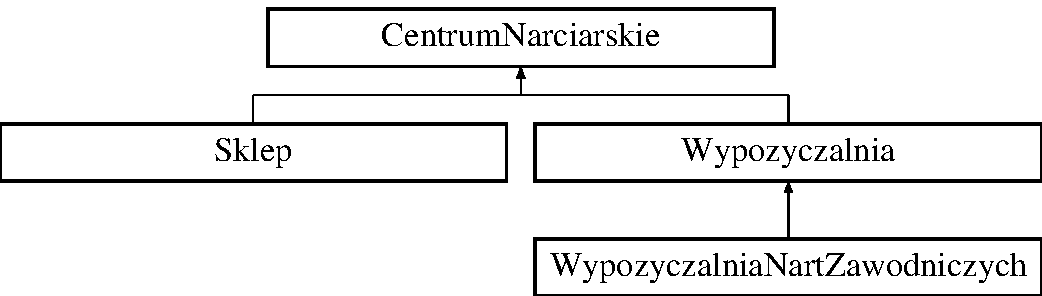
\includegraphics[height=3.000000cm]{class_centrum_narciarskie}
\end{center}
\end{figure}
\subsection*{Metody publiczne}
\begin{DoxyCompactItemize}
\item 
\mbox{\Hypertarget{class_centrum_narciarskie_aa355c508b58fddb6b3bcaed4c25b48ef}\label{class_centrum_narciarskie_aa355c508b58fddb6b3bcaed4c25b48ef}} 
virtual void {\bfseries zmien\+Ilosc\+Pomieszczen} (unsigned int iloscpomieszczen)=0
\item 
\mbox{\Hypertarget{class_centrum_narciarskie_a15784c30d71940ca8175ec08017c5cef}\label{class_centrum_narciarskie_a15784c30d71940ca8175ec08017c5cef}} 
virtual void {\bfseries wypisz\+Wszystko} ()=0
\end{DoxyCompactItemize}
\subsection*{Atrybuty chronione}
\begin{DoxyCompactItemize}
\item 
\mbox{\Hypertarget{class_centrum_narciarskie_a671a12e1f05ad515f1d34674d475089b}\label{class_centrum_narciarskie_a671a12e1f05ad515f1d34674d475089b}} 
string {\bfseries typ\+\_\+lokalu}
\item 
\mbox{\Hypertarget{class_centrum_narciarskie_aeb2c143fb961e8a7a1ef5440bf47b22f}\label{class_centrum_narciarskie_aeb2c143fb961e8a7a1ef5440bf47b22f}} 
string {\bfseries adres}
\item 
\mbox{\Hypertarget{class_centrum_narciarskie_a8081f1fcecfec0e8052b8f600d5cdffd}\label{class_centrum_narciarskie_a8081f1fcecfec0e8052b8f600d5cdffd}} 
unsigned int {\bfseries pomieszczenia}
\end{DoxyCompactItemize}


Dokumentacja dla tej klasy została wygenerowana z plików\+:\begin{DoxyCompactItemize}
\item 
centrumnarciarskie.\+hpp\item 
centrumnarciarskie.\+cpp\end{DoxyCompactItemize}

\hypertarget{class_kask}{}\section{Dokumentacja klasy Kask}
\label{class_kask}\index{Kask@{Kask}}
\subsection*{Metody publiczne}
\begin{DoxyCompactItemize}
\item 
\mbox{\Hypertarget{class_kask_a9d6f69168af42010ca3009547bd8ff43}\label{class_kask_a9d6f69168af42010ca3009547bd8ff43}} 
{\bfseries Kask} (string)
\item 
\mbox{\Hypertarget{class_kask_ab2e0a0ee02645eb1f5f3ce1a5671d2d0}\label{class_kask_ab2e0a0ee02645eb1f5f3ce1a5671d2d0}} 
{\bfseries Kask} (string, unsigned int, unsigned int, Kolor\+\_\+k)
\item 
\mbox{\Hypertarget{class_kask_a95c8969d275dbcd7693eb974daddb6ee}\label{class_kask_a95c8969d275dbcd7693eb974daddb6ee}} 
{\bfseries Kask} (const \hyperlink{class_kask}{Kask} \&kask)
\item 
\mbox{\Hypertarget{class_kask_ab1aee9ce929f776824c3931ab236cb69}\label{class_kask_ab1aee9ce929f776824c3931ab236cb69}} 
string {\bfseries zwroc\+Nazwa} ()
\item 
\mbox{\Hypertarget{class_kask_a24199eaad772b42465c66692b8edfa99}\label{class_kask_a24199eaad772b42465c66692b8edfa99}} 
unsigned int {\bfseries zwroc\+Cena} ()
\item 
\mbox{\Hypertarget{class_kask_a4682c0f3f1b9fce124d4d81bff19ff92}\label{class_kask_a4682c0f3f1b9fce124d4d81bff19ff92}} 
unsigned int {\bfseries zwroc\+Srednica} ()
\item 
\mbox{\Hypertarget{class_kask_a20878029169fa45fd4499abd8374b3d5}\label{class_kask_a20878029169fa45fd4499abd8374b3d5}} 
string {\bfseries zwroc\+Kolor} (void)
\item 
\mbox{\Hypertarget{class_kask_a9c31b947c5304758b8c1382404f239db}\label{class_kask_a9c31b947c5304758b8c1382404f239db}} 
Kolor\+\_\+k {\bfseries zwroc\+KolorN} (void) const
\item 
\mbox{\Hypertarget{class_kask_a89eb4c4acdc0b143bdfd8837d7bbb502}\label{class_kask_a89eb4c4acdc0b143bdfd8837d7bbb502}} 
void {\bfseries zmien\+Nazwe} (string k\+\_\+nazwa)
\item 
\mbox{\Hypertarget{class_kask_a5782fca051e92ff55d484e3ebbcdb9a3}\label{class_kask_a5782fca051e92ff55d484e3ebbcdb9a3}} 
void {\bfseries zmien\+Cene} (unsigned int k\+\_\+cena)
\item 
\mbox{\Hypertarget{class_kask_abb8614360e4958220a4f779faac7393a}\label{class_kask_abb8614360e4958220a4f779faac7393a}} 
bool {\bfseries operator==} (const \hyperlink{class_kask}{Kask} \&kask)
\item 
\mbox{\Hypertarget{class_kask_a429e0cf2f819de1b68b9a57f4760ca80}\label{class_kask_a429e0cf2f819de1b68b9a57f4760ca80}} 
bool {\bfseries operator$<$$<$} (const \hyperlink{class_kask}{Kask} \&kask)
\item 
\mbox{\Hypertarget{class_kask_a49180364c9192e95934c67b9360b2c87}\label{class_kask_a49180364c9192e95934c67b9360b2c87}} 
void {\bfseries operator=} (const \hyperlink{class_kask}{Kask} \&kask)
\end{DoxyCompactItemize}
\subsection*{Statyczne metody publiczne}
\begin{DoxyCompactItemize}
\item 
\mbox{\Hypertarget{class_kask_aaaadafb0131fe2381d4e71696145734c}\label{class_kask_aaaadafb0131fe2381d4e71696145734c}} 
static size\+\_\+t {\bfseries zwroc\+Ilosc\+Kaskow} (void)
\end{DoxyCompactItemize}


Dokumentacja dla tej klasy została wygenerowana z plików\+:\begin{DoxyCompactItemize}
\item 
kask.\+hpp\item 
kask.\+cpp\end{DoxyCompactItemize}

\hypertarget{class_narty}{}\section{Dokumentacja klasy Narty}
\label{class_narty}\index{Narty@{Narty}}
\subsection*{Metody publiczne}
\begin{DoxyCompactItemize}
\item 
\mbox{\Hypertarget{class_narty_a0e97c71362fec6e6495f35750e1c45d2}\label{class_narty_a0e97c71362fec6e6495f35750e1c45d2}} 
{\bfseries Narty} (string)
\item 
\mbox{\Hypertarget{class_narty_a061922fefe4e2cc8da8daf66ce0070fd}\label{class_narty_a061922fefe4e2cc8da8daf66ce0070fd}} 
{\bfseries Narty} (string, unsigned int, unsigned int, Poziom\+\_\+n, Dostepnosc\+\_\+n)
\item 
\mbox{\Hypertarget{class_narty_af5629023cde81ccb70cef0d02d315347}\label{class_narty_af5629023cde81ccb70cef0d02d315347}} 
{\bfseries Narty} (const \hyperlink{class_narty}{Narty} \&narty)
\item 
\mbox{\Hypertarget{class_narty_a704912bf1923302796ed7465678d4664}\label{class_narty_a704912bf1923302796ed7465678d4664}} 
string {\bfseries zwroc\+Nazwa} () const
\item 
\mbox{\Hypertarget{class_narty_a417482bac2097c29ce9c74c721ba7854}\label{class_narty_a417482bac2097c29ce9c74c721ba7854}} 
unsigned int {\bfseries zwroc\+Cena} () const
\item 
\mbox{\Hypertarget{class_narty_a16205402be7796d3bbdbb9b7eb34507f}\label{class_narty_a16205402be7796d3bbdbb9b7eb34507f}} 
unsigned int {\bfseries zwroc\+Dlugosc} () const
\item 
\mbox{\Hypertarget{class_narty_a9e9f486ea6e7aee2b3ea765bb8c126c1}\label{class_narty_a9e9f486ea6e7aee2b3ea765bb8c126c1}} 
string {\bfseries zwroc\+Poziom} (void) const
\item 
\mbox{\Hypertarget{class_narty_a81d3658a9d8f0db31e469516efd7e7a3}\label{class_narty_a81d3658a9d8f0db31e469516efd7e7a3}} 
string {\bfseries zwroc\+Dostepnosc} (void) const
\item 
\mbox{\Hypertarget{class_narty_a28ea4239352274779d53b5ecaf137fff}\label{class_narty_a28ea4239352274779d53b5ecaf137fff}} 
Poziom\+\_\+n {\bfseries zwroc\+PoziomN} (void) const
\item 
\mbox{\Hypertarget{class_narty_a72e89246e4552434b12d514f80a60e64}\label{class_narty_a72e89246e4552434b12d514f80a60e64}} 
Dostepnosc\+\_\+n {\bfseries zwroc\+DostepnoscN} (void) const
\item 
\mbox{\Hypertarget{class_narty_a35747349d49dc91ff1ac414dcf93a3ad}\label{class_narty_a35747349d49dc91ff1ac414dcf93a3ad}} 
void {\bfseries zmien\+Nazwe} (string n\+\_\+nazwa)
\item 
\mbox{\Hypertarget{class_narty_a88225c95156e51dc84d9ddc50a92989f}\label{class_narty_a88225c95156e51dc84d9ddc50a92989f}} 
void {\bfseries zmien\+Cene} (unsigned int n\+\_\+cena)
\item 
\mbox{\Hypertarget{class_narty_af3f12c0fc248e86f0a9f447edeacbba8}\label{class_narty_af3f12c0fc248e86f0a9f447edeacbba8}} 
void {\bfseries zmien\+Wszystko} (string nazwa\+\_\+s, unsigned int cena\+\_\+s, unsigned int dlugosc\+\_\+s, Poziom\+\_\+n poziom\+\_\+s, Dostepnosc\+\_\+n dostepnosc\+\_\+s)
\item 
\mbox{\Hypertarget{class_narty_a18cc9d232e226a63ca1b95d9afd7b1e3}\label{class_narty_a18cc9d232e226a63ca1b95d9afd7b1e3}} 
void {\bfseries operator=} (const \hyperlink{class_narty}{Narty} \&narty)
\item 
\mbox{\Hypertarget{class_narty_a74cd13f61fc4bffea616367961391d54}\label{class_narty_a74cd13f61fc4bffea616367961391d54}} 
bool {\bfseries operator==} (const \hyperlink{class_narty}{Narty} \&narty)
\item 
\mbox{\Hypertarget{class_narty_abd4a3b0f020a2ae9d65668e9dca26d65}\label{class_narty_abd4a3b0f020a2ae9d65668e9dca26d65}} 
bool {\bfseries operator$<$} (const \hyperlink{class_narty}{Narty} \&narty)
\item 
\mbox{\Hypertarget{class_narty_abd3b42f980291b55ea35e49091aec194}\label{class_narty_abd3b42f980291b55ea35e49091aec194}} 
bool {\bfseries operator$>$} (const \hyperlink{class_narty}{Narty} \&narty)
\item 
\mbox{\Hypertarget{class_narty_a412b7395ba583848b6803d65f747bcb9}\label{class_narty_a412b7395ba583848b6803d65f747bcb9}} 
bool {\bfseries operator!=} (const \hyperlink{class_narty}{Narty} \&narty)
\item 
\mbox{\Hypertarget{class_narty_ac18fc5685a7dd1c3fd7e8be18edf869f}\label{class_narty_ac18fc5685a7dd1c3fd7e8be18edf869f}} 
bool {\bfseries operator$^\wedge$} (const \hyperlink{class_narty}{Narty} \&narty)
\item 
\mbox{\Hypertarget{class_narty_a06af67856b6e340325ea906469eec6bd}\label{class_narty_a06af67856b6e340325ea906469eec6bd}} 
\hyperlink{class_narty}{Narty} {\bfseries operator+} (const \hyperlink{class_narty}{Narty} \&narty)
\end{DoxyCompactItemize}
\subsection*{Statyczne metody publiczne}
\begin{DoxyCompactItemize}
\item 
\mbox{\Hypertarget{class_narty_a2f7178d88af8a1939ffa0c546b3ac4ee}\label{class_narty_a2f7178d88af8a1939ffa0c546b3ac4ee}} 
static size\+\_\+t {\bfseries zwroc\+Ilosc\+Nart} (void)
\end{DoxyCompactItemize}
\subsection*{Przyjaciele}
\begin{DoxyCompactItemize}
\item 
\mbox{\Hypertarget{class_narty_af8090f0e17f1b341d4ef1e4c55391edf}\label{class_narty_af8090f0e17f1b341d4ef1e4c55391edf}} 
ostream \& {\bfseries operator$<$$<$} (ostream \&os, const \hyperlink{class_narty}{Narty} \&narty)
\end{DoxyCompactItemize}


Dokumentacja dla tej klasy została wygenerowana z plików\+:\begin{DoxyCompactItemize}
\item 
narty.\+hpp\item 
narty.\+cpp\end{DoxyCompactItemize}

\hypertarget{class_sklep}{}\section{Dokumentacja klasy Sklep}
\label{class_sklep}\index{Sklep@{Sklep}}
Diagram dziedziczenia dla Sklep\begin{figure}[H]
\begin{center}
\leavevmode
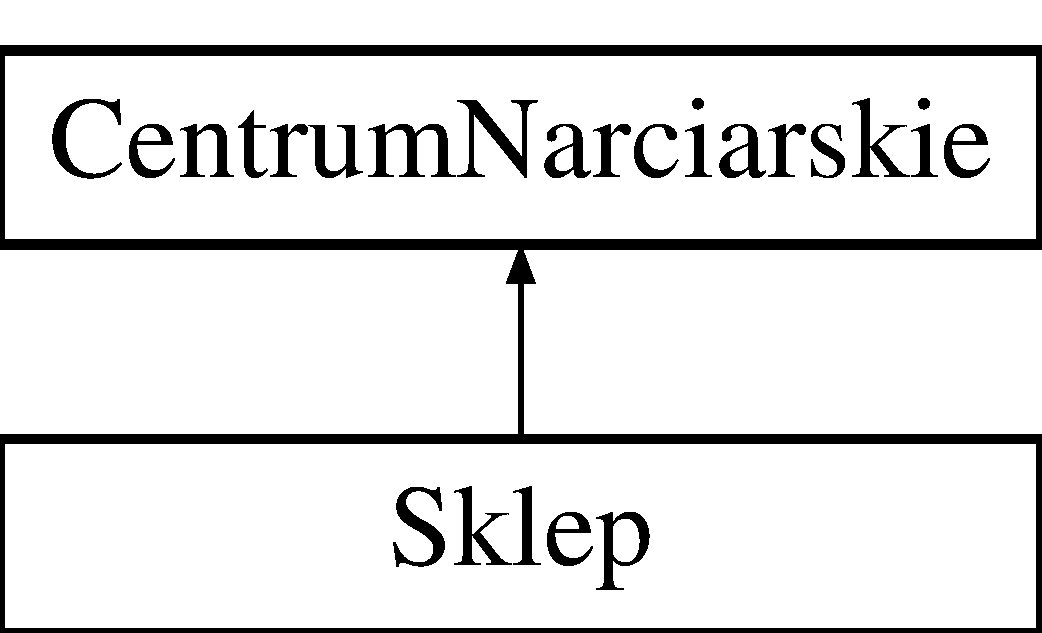
\includegraphics[height=2.000000cm]{class_sklep}
\end{center}
\end{figure}
\subsection*{Metody publiczne}
\begin{DoxyCompactItemize}
\item 
\mbox{\Hypertarget{class_sklep_a13a92e8796513fb8dcfaad878b55bb65}\label{class_sklep_a13a92e8796513fb8dcfaad878b55bb65}} 
void {\bfseries wypisz\+Wszystko} ()
\item 
\mbox{\Hypertarget{class_sklep_a2a21b324f47f33722d0d3ce96c6e2084}\label{class_sklep_a2a21b324f47f33722d0d3ce96c6e2084}} 
void {\bfseries zmien\+Ilosc\+Pomieszczen} (unsigned int iloscpomieszczen)
\end{DoxyCompactItemize}
\subsection*{Dodatkowe Dziedziczone Składowe}


Dokumentacja dla tej klasy została wygenerowana z plików\+:\begin{DoxyCompactItemize}
\item 
sklep.\+hpp\item 
sklep.\+cpp\end{DoxyCompactItemize}

\hypertarget{class_snowboard}{}\section{Dokumentacja klasy Snowboard}
\label{class_snowboard}\index{Snowboard@{Snowboard}}
\subsection*{Metody publiczne}
\begin{DoxyCompactItemize}
\item 
\mbox{\Hypertarget{class_snowboard_aeede8444cd911d37088be24d03113ae9}\label{class_snowboard_aeede8444cd911d37088be24d03113ae9}} 
{\bfseries Snowboard} (string)
\item 
\mbox{\Hypertarget{class_snowboard_a6d4fae152cd7428a443d101605eaa24a}\label{class_snowboard_a6d4fae152cd7428a443d101605eaa24a}} 
{\bfseries Snowboard} (string, unsigned int, unsigned int, Poziom\+\_\+s, Dostepnosc\+\_\+s)
\item 
\mbox{\Hypertarget{class_snowboard_adb570913caa563993262d3370a2750eb}\label{class_snowboard_adb570913caa563993262d3370a2750eb}} 
{\bfseries Snowboard} (const \hyperlink{class_snowboard}{Snowboard} \&snowboard)
\item 
\mbox{\Hypertarget{class_snowboard_abfcf3dd0c6af65f187f5e6bf0dea9c0d}\label{class_snowboard_abfcf3dd0c6af65f187f5e6bf0dea9c0d}} 
string {\bfseries zwroc\+Nazwa} ()
\item 
\mbox{\Hypertarget{class_snowboard_aa402c2e023feffd7f5ae0d1e2c039d3e}\label{class_snowboard_aa402c2e023feffd7f5ae0d1e2c039d3e}} 
unsigned int {\bfseries zwroc\+Cena} ()
\item 
\mbox{\Hypertarget{class_snowboard_a169ebefeb57f45826056b0850e3b8701}\label{class_snowboard_a169ebefeb57f45826056b0850e3b8701}} 
unsigned int {\bfseries zwroc\+Dlugosc} ()
\item 
\mbox{\Hypertarget{class_snowboard_adbe3f6f995981479d7aed1b23f5b4357}\label{class_snowboard_adbe3f6f995981479d7aed1b23f5b4357}} 
string {\bfseries zwroc\+Poziom} (void)
\item 
\mbox{\Hypertarget{class_snowboard_a393b5795787fecd229e683fee5ffc5e4}\label{class_snowboard_a393b5795787fecd229e683fee5ffc5e4}} 
string {\bfseries zwroc\+Dostepnosc} (void)
\item 
\mbox{\Hypertarget{class_snowboard_a42e01d1ddae44085d414490e110ed945}\label{class_snowboard_a42e01d1ddae44085d414490e110ed945}} 
Poziom\+\_\+s {\bfseries zwroc\+PoziomN} (void) const
\item 
\mbox{\Hypertarget{class_snowboard_aaa30ba4f895aebff920ac25c5d477fd8}\label{class_snowboard_aaa30ba4f895aebff920ac25c5d477fd8}} 
Dostepnosc\+\_\+s {\bfseries zwroc\+DostepnoscN} (void) const
\item 
\mbox{\Hypertarget{class_snowboard_a82357c21c3b6db16705afc871e79ee55}\label{class_snowboard_a82357c21c3b6db16705afc871e79ee55}} 
void {\bfseries zmien\+Nazwe} (string s\+\_\+nazwa)
\item 
\mbox{\Hypertarget{class_snowboard_a4a85e0a9b666ec2684bd924fb462948e}\label{class_snowboard_a4a85e0a9b666ec2684bd924fb462948e}} 
void {\bfseries zmien\+Cene} (unsigned int s\+\_\+cena)
\item 
\mbox{\Hypertarget{class_snowboard_aa8da85ff612a1916b31a281b54a134cc}\label{class_snowboard_aa8da85ff612a1916b31a281b54a134cc}} 
bool {\bfseries operator==} (const \hyperlink{class_snowboard}{Snowboard} \&snowboard)
\item 
\mbox{\Hypertarget{class_snowboard_a86c206599d92e0c7b63afc3d4d2d5393}\label{class_snowboard_a86c206599d92e0c7b63afc3d4d2d5393}} 
bool {\bfseries operator$<$$<$} (const \hyperlink{class_snowboard}{Snowboard} \&snowboard)
\item 
\mbox{\Hypertarget{class_snowboard_a1dc59ff0f8644e8aadae2c08fecde3d0}\label{class_snowboard_a1dc59ff0f8644e8aadae2c08fecde3d0}} 
bool {\bfseries operator$>$$>$} (const \hyperlink{class_snowboard}{Snowboard} \&snowboard)
\item 
\mbox{\Hypertarget{class_snowboard_ad1d481630326c8bea93090791efef496}\label{class_snowboard_ad1d481630326c8bea93090791efef496}} 
void {\bfseries operator=} (const \hyperlink{class_snowboard}{Snowboard} \&snowboard)
\end{DoxyCompactItemize}
\subsection*{Statyczne metody publiczne}
\begin{DoxyCompactItemize}
\item 
\mbox{\Hypertarget{class_snowboard_a424d6bd96d0949bc254bd696cbb1c6cb}\label{class_snowboard_a424d6bd96d0949bc254bd696cbb1c6cb}} 
static size\+\_\+t {\bfseries zwroc\+Ilosc\+Snowboardow} (void)
\end{DoxyCompactItemize}


Dokumentacja dla tej klasy została wygenerowana z plików\+:\begin{DoxyCompactItemize}
\item 
snowboard.\+hpp\item 
snowboard.\+cpp\end{DoxyCompactItemize}

\hypertarget{class_wypozyczalnia}{}\section{Dokumentacja klasy Wypozyczalnia}
\label{class_wypozyczalnia}\index{Wypozyczalnia@{Wypozyczalnia}}
Diagram dziedziczenia dla Wypozyczalnia\begin{figure}[H]
\begin{center}
\leavevmode
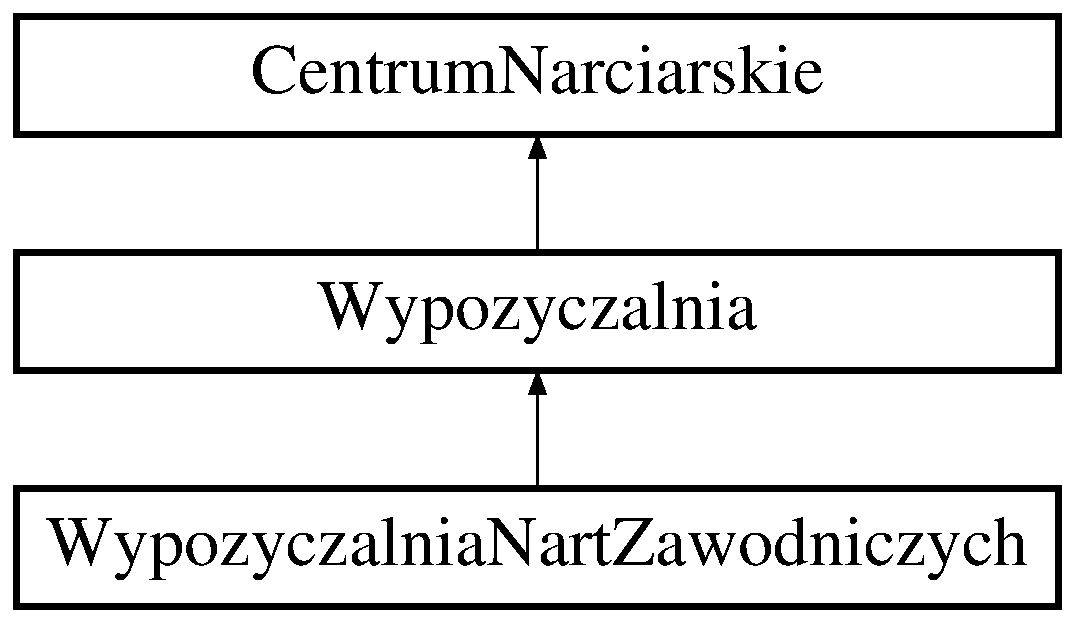
\includegraphics[height=3.000000cm]{class_wypozyczalnia}
\end{center}
\end{figure}
\subsection*{Metody publiczne}
\begin{DoxyCompactItemize}
\item 
\mbox{\Hypertarget{class_wypozyczalnia_afa521c8f4087a3587af1597de6d1d67c}\label{class_wypozyczalnia_afa521c8f4087a3587af1597de6d1d67c}} 
{\bfseries Wypozyczalnia} (string, unsigned int)
\item 
\mbox{\Hypertarget{class_wypozyczalnia_aef0b87f9ab0a39e8384e48d3d80503ad}\label{class_wypozyczalnia_aef0b87f9ab0a39e8384e48d3d80503ad}} 
{\bfseries Wypozyczalnia} (const \hyperlink{class_wypozyczalnia}{Wypozyczalnia} \&wypozyczalnia)
\item 
\mbox{\Hypertarget{class_wypozyczalnia_ad341700b6cfc7de365475a210b2a9bdb}\label{class_wypozyczalnia_ad341700b6cfc7de365475a210b2a9bdb}} 
void {\bfseries zmien\+Ilosc\+Pomieszczen} (unsigned int iloscpomieszczen)
\item 
\mbox{\Hypertarget{class_wypozyczalnia_a1de447b411ead2785381ee0293937a32}\label{class_wypozyczalnia_a1de447b411ead2785381ee0293937a32}} 
void {\bfseries dodaj\+Narty} (string nazwa\+\_\+s)
\item 
\mbox{\Hypertarget{class_wypozyczalnia_ac7adef1f4f60b4b99a8853910936fc5e}\label{class_wypozyczalnia_ac7adef1f4f60b4b99a8853910936fc5e}} 
void {\bfseries dodaj\+Narty} (string nazwa\+\_\+s, unsigned int cena\+\_\+s, unsigned int dlugosc\+\_\+s, Poziom\+\_\+n poziom\+\_\+s, Dostepnosc\+\_\+n dostepnosc\+\_\+s)
\item 
\mbox{\Hypertarget{class_wypozyczalnia_a09beac2dbecfae112a9ea873485218bd}\label{class_wypozyczalnia_a09beac2dbecfae112a9ea873485218bd}} 
void {\bfseries wypisz\+Wszystko} ()
\item 
\mbox{\Hypertarget{class_wypozyczalnia_a47b50362048a34c2be7de80d9fc79b26}\label{class_wypozyczalnia_a47b50362048a34c2be7de80d9fc79b26}} 
virtual int {\bfseries liczba\+Nart} ()
\item 
\mbox{\Hypertarget{class_wypozyczalnia_a23adfc6602609355a82a9597b6e27d14}\label{class_wypozyczalnia_a23adfc6602609355a82a9597b6e27d14}} 
void {\bfseries usun\+Narte} (string nazwa\+\_\+n)
\item 
\mbox{\Hypertarget{class_wypozyczalnia_a0ca06cb1a024785c467b90f4c0c1ce39}\label{class_wypozyczalnia_a0ca06cb1a024785c467b90f4c0c1ce39}} 
void {\bfseries operator+} (string nazwa\+\_\+s)
\end{DoxyCompactItemize}
\subsection*{Statyczne metody publiczne}
\begin{DoxyCompactItemize}
\item 
\mbox{\Hypertarget{class_wypozyczalnia_a98cc31471aaf1bedc8c194b8aed569fa}\label{class_wypozyczalnia_a98cc31471aaf1bedc8c194b8aed569fa}} 
static size\+\_\+t {\bfseries zwroc\+Ilosc\+Wypozyczalni} (void)
\item 
\mbox{\Hypertarget{class_wypozyczalnia_a032fa06c91b8387bd88a8c8327fa285b}\label{class_wypozyczalnia_a032fa06c91b8387bd88a8c8327fa285b}} 
static size\+\_\+t {\bfseries zwroc\+Ilosc\+Nart} (void)
\end{DoxyCompactItemize}
\subsection*{Dodatkowe Dziedziczone Składowe}


Dokumentacja dla tej klasy została wygenerowana z plików\+:\begin{DoxyCompactItemize}
\item 
wypozyczalnia.\+hpp\item 
wypozyczalnia.\+cpp\end{DoxyCompactItemize}

\hypertarget{class_wypozyczalnia_nart_zawodniczych}{}\section{Dokumentacja klasy Wypozyczalnia\+Nart\+Zawodniczych}
\label{class_wypozyczalnia_nart_zawodniczych}\index{Wypozyczalnia\+Nart\+Zawodniczych@{Wypozyczalnia\+Nart\+Zawodniczych}}
Diagram dziedziczenia dla Wypozyczalnia\+Nart\+Zawodniczych\begin{figure}[H]
\begin{center}
\leavevmode
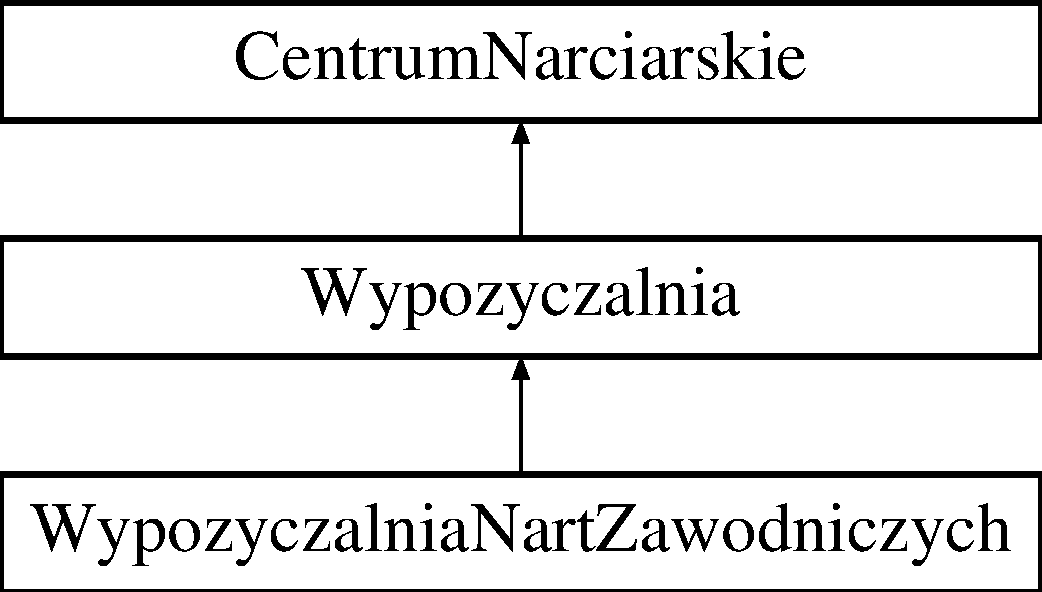
\includegraphics[height=3.000000cm]{class_wypozyczalnia_nart_zawodniczych}
\end{center}
\end{figure}
\subsection*{Metody publiczne}
\begin{DoxyCompactItemize}
\item 
\mbox{\Hypertarget{class_wypozyczalnia_nart_zawodniczych_a9c339169c48d6e6ef8310494cbfcf8de}\label{class_wypozyczalnia_nart_zawodniczych_a9c339169c48d6e6ef8310494cbfcf8de}} 
void {\bfseries dodaj\+Narty} (string nazwa\+\_\+s)
\item 
\mbox{\Hypertarget{class_wypozyczalnia_nart_zawodniczych_a2bc434fdfbb3b3e48d063f7ca56c76be}\label{class_wypozyczalnia_nart_zawodniczych_a2bc434fdfbb3b3e48d063f7ca56c76be}} 
void \hyperlink{class_wypozyczalnia_nart_zawodniczych_a2bc434fdfbb3b3e48d063f7ca56c76be}{wypisz\+Wszystko} ()
\begin{DoxyCompactList}\small\item\em funkcja wirtualna wypisujaca cechy danego obiektu \end{DoxyCompactList}\item 
\mbox{\Hypertarget{class_wypozyczalnia_nart_zawodniczych_a074ccb9dbe9b8be619053d0ed69edf26}\label{class_wypozyczalnia_nart_zawodniczych_a074ccb9dbe9b8be619053d0ed69edf26}} 
void \hyperlink{class_wypozyczalnia_nart_zawodniczych_a074ccb9dbe9b8be619053d0ed69edf26}{wypisz\+Zapisane} ()
\begin{DoxyCompactList}\small\item\em funkcj wirtualna wypisujaca wczytane obiekty \end{DoxyCompactList}\item 
\mbox{\Hypertarget{class_wypozyczalnia_nart_zawodniczych_adc1ebefbce7393486ccd50ba3274b804}\label{class_wypozyczalnia_nart_zawodniczych_adc1ebefbce7393486ccd50ba3274b804}} 
int \hyperlink{class_wypozyczalnia_nart_zawodniczych_adc1ebefbce7393486ccd50ba3274b804}{liczba\+Nart} ()
\begin{DoxyCompactList}\small\item\em funkcja wirtualna wypisujaca liczbe nart \end{DoxyCompactList}\item 
\mbox{\Hypertarget{class_wypozyczalnia_nart_zawodniczych_a84b33d3eb8f2c2889866207afa4f74e3}\label{class_wypozyczalnia_nart_zawodniczych_a84b33d3eb8f2c2889866207afa4f74e3}} 
void \hyperlink{class_wypozyczalnia_nart_zawodniczych_a84b33d3eb8f2c2889866207afa4f74e3}{zapisz} (\hyperlink{class_wypozyczalnia_nart_zawodniczych}{Wypozyczalnia\+Nart\+Zawodniczych} \&wypozyczalniaZ)
\begin{DoxyCompactList}\small\item\em funkcja sluzaca do zapisu Wypozyczalni nart zawodniczych \end{DoxyCompactList}\item 
\mbox{\Hypertarget{class_wypozyczalnia_nart_zawodniczych_a1a7c5b253967d7c214b68f0e27273c91}\label{class_wypozyczalnia_nart_zawodniczych_a1a7c5b253967d7c214b68f0e27273c91}} 
void \hyperlink{class_wypozyczalnia_nart_zawodniczych_a1a7c5b253967d7c214b68f0e27273c91}{wczytaj} (\hyperlink{class_wypozyczalnia_nart_zawodniczych}{Wypozyczalnia\+Nart\+Zawodniczych} \&wypozyczalniaZ)
\begin{DoxyCompactList}\small\item\em funkcja sluzaca do wczytywania Wypozyczalni nart zawodniczych \end{DoxyCompactList}\end{DoxyCompactItemize}
\subsection*{Przyjaciele}
\begin{DoxyCompactItemize}
\item 
\mbox{\Hypertarget{class_wypozyczalnia_nart_zawodniczych_ab8dabbf7f792bd7e412f063fee53d7ce}\label{class_wypozyczalnia_nart_zawodniczych_ab8dabbf7f792bd7e412f063fee53d7ce}} 
ostream \& \hyperlink{class_wypozyczalnia_nart_zawodniczych_ab8dabbf7f792bd7e412f063fee53d7ce}{operator$<$$<$} (ostream \&w, \hyperlink{class_wypozyczalnia_nart_zawodniczych}{Wypozyczalnia\+Nart\+Zawodniczych} \&wypozyczalniaZ)
\begin{DoxyCompactList}\small\item\em operator strumieniowy do zapisu \end{DoxyCompactList}\item 
\mbox{\Hypertarget{class_wypozyczalnia_nart_zawodniczych_a12481b91994af65722e631c2470457e1}\label{class_wypozyczalnia_nart_zawodniczych_a12481b91994af65722e631c2470457e1}} 
istream \& \hyperlink{class_wypozyczalnia_nart_zawodniczych_a12481b91994af65722e631c2470457e1}{operator$>$$>$} (istream \&w, \hyperlink{class_wypozyczalnia_nart_zawodniczych}{Wypozyczalnia\+Nart\+Zawodniczych} \&wypozyczalniaZ)
\begin{DoxyCompactList}\small\item\em operator strumieniowy do wczytywania \end{DoxyCompactList}\end{DoxyCompactItemize}
\subsection*{Dodatkowe Dziedziczone Składowe}


Dokumentacja dla tej klasy została wygenerowana z plików\+:\begin{DoxyCompactItemize}
\item 
wypnartzawod.\+hpp\item 
wypnartzawod.\+cpp\end{DoxyCompactItemize}

%--- End generated contents ---

% Index
\backmatter
\newpage
\phantomsection
\clearemptydoublepage
\addcontentsline{toc}{chapter}{Indeks}
\printindex

\end{document}
